\section{Introduction}
In recent years, there has been a growing concern about the increasing number of fatalities caused by car accidents resulting from driver distraction. According to the World Health Organization~(WHO), driver distraction is a major contributing factor to road traffic accidents worldwide. In the U.S., approximately 30\% were observed to perform secondary tasks while driving~\cite{who2011driver}. In the European Union, it's estimated that driver distraction is a contributing factor in 44\% of collisions~\cite{adminaite2021road}.
%Therefore distracted driving has become a leading cause of accidents, accounting for a significant portion of road fatalities worldwide. This alarming trend has necessitated the development of advanced algorithms capable of recognizing driver actions and behaviors to prevent such accidents and promote road safety. 
To address this critical issue, there has been a surge in the development of activity recognition systems specifically tailored for the car interior. These systems aim to identify and analyze various driver activities, such as hand gestures, head movements, and body postures, in real-time. 
%By accurately recognizing these actions, potential distractions and unsafe behaviors can be identified, allowing for timely intervention and accident prevention. 


\begin{figure}[t]
      \centering
      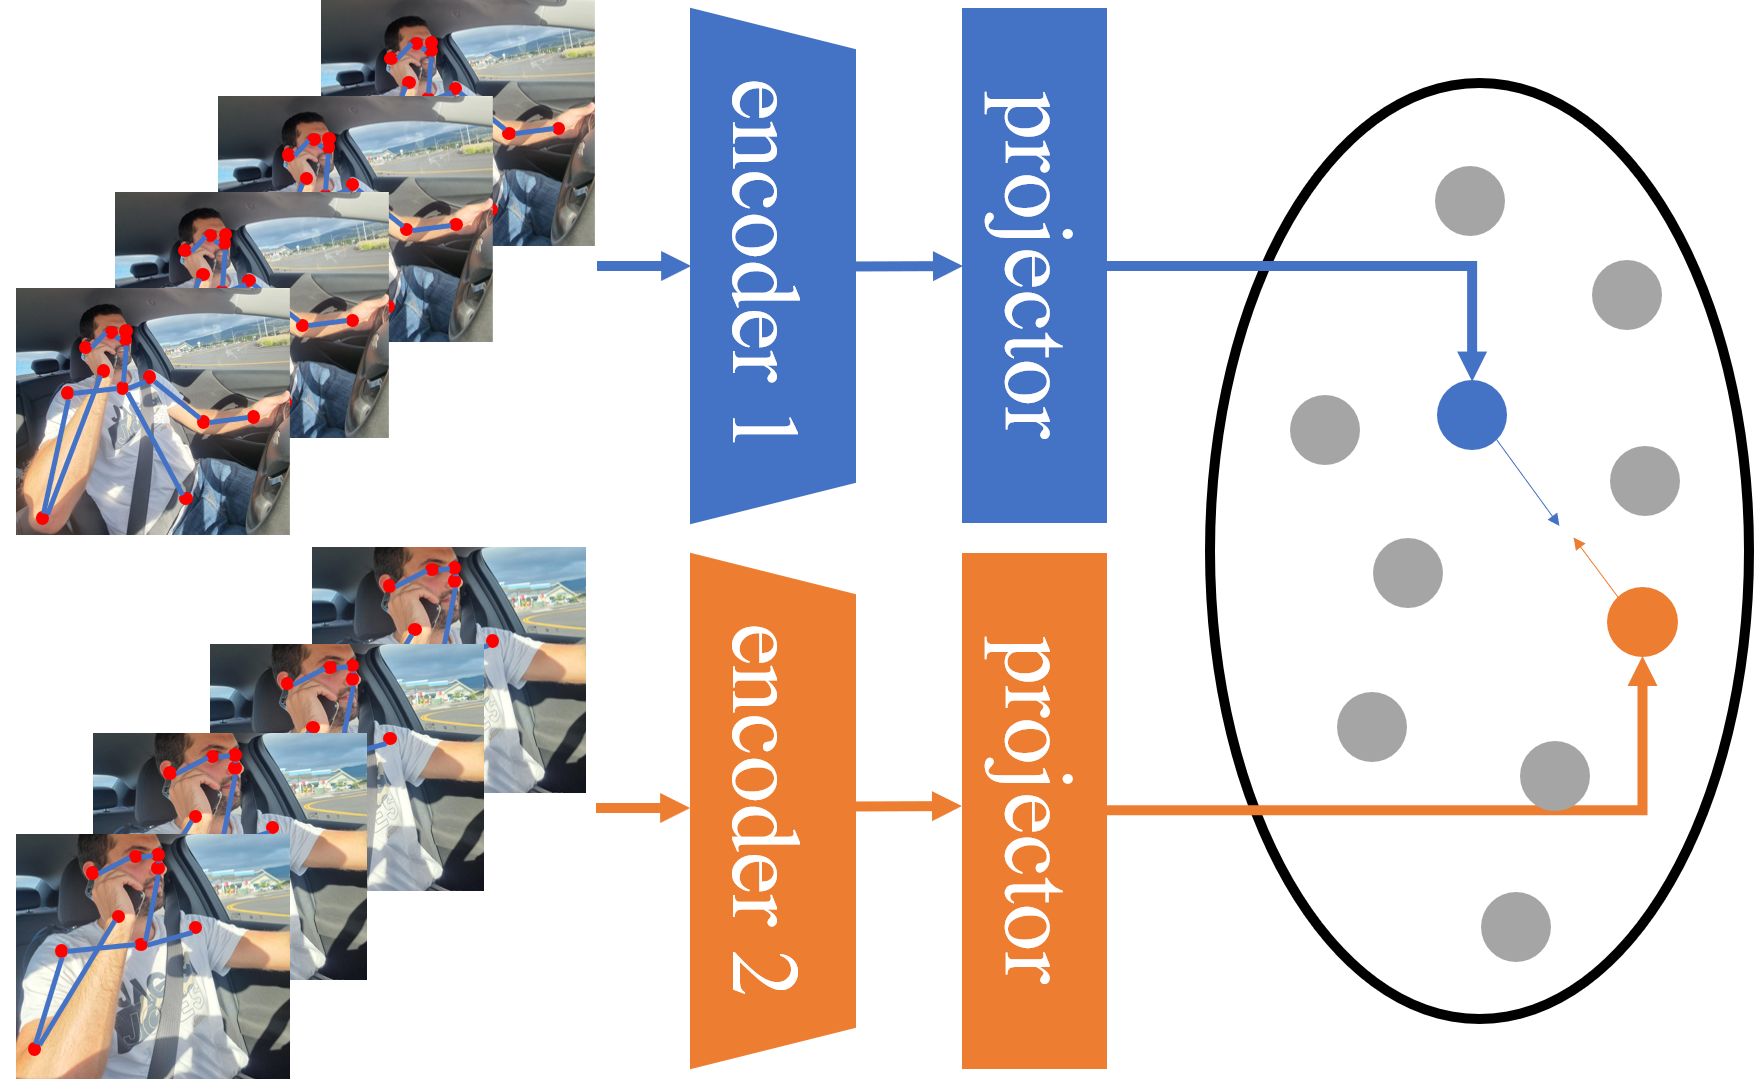
\includegraphics[width=\linewidth]{figures/darssl.png}
      \caption{Principle of a 3D skeleton-based contrastive self-supervised learning approach without negative samples for driver activity recognition. It consists of a two encoders. Different augmentations of the same sample are input to the encoders.}
      \label{fig:darssl}
\end{figure}


Traditional supervised learning methods have been widely employed for activity recognition tasks. However, they heavily rely on annotated datasets, which are costly and time-consuming to produce. 
%Annotated datasets require manual labeling of each action instance, posing practical limitations when it comes to scaling up the training process. To overcome these challenges, self-supervised learning has emerged as a promising alternative approach. 
Unlike traditional supervised learning, self-supervised learning leverages label-free data to learn meaningful representations. In the context of these challenges and opportunities, this study aims to enhance vehicle interior activity recognition by leveraging contrastive self-supervised learning techniques with 3D driver skeleton representations. 
%By utilizing label-free data, this approach can effectively learn informative representations that capture the nuances of driver actions in the car interior. 
Through extensive experimentation and evaluation, we seek to demonstrate the effectiveness of contrastive self-supervised learning with 3D driver skeleton representations in improving the accuracy and robustness of in-cabin activity recognition systems. 

Human activity recognition has been extensively studied using different modalities, such as RGB videos or depth cameras. However, these modalities often come with significant computational costs, making them less suitable for resource-constrained environments. 
%In response to this challenge, human skeleton data has emerged as a promising alternative. 
Skeleton data offers a more efficient representation of human activities, reducing the computational complexity and storage requirements. They also provide a lightweight and efficient alternative that not only reduces computational overhead but also offers the potential to generalize across domains, enabling broader applicability in real-world scenarios. While self-supervised learning has shown promise in various domains, its application to skeleton-based driver activity recognition is still in its early stages. Further research and investigations are necessary to explore the full potential of self-supervised learning in this context. With our work we contribute to this exploration of self-supervised 3D skeleton-based driver activity recognition.

Furthermore, the lack of large activity recognition datasets specifically dedicated to driver behavior inside the car presents another challenge. Existing datasets often focus on general activity recognition but fail to capture the nuanced activities and behaviors specific to drivers within the vehicle environment. To address this gap, we will focus on the test and evaluation on the Drive\&Act dataset \cite{drive_and_act_2019_iccv} tailored specifically to driver behavior inside the car. This dedicated dataset incorporates a wide range of driver activities and behaviors, providing a realistic and comprehensive evaluation platform for activity recognition algorithms in the automotive context. 
%This dataset uniquely facilitates research on activity recognition under realistic driving conditions, incorporating factors like low illumination and limited body visibility. By addressing these practical challenges, our research aims to provide insights into the models' adaptability to real-world scenarios, ultimately contributing to the development of more effective and resilient action recognition systems for in-vehicle environments.
%The first research objective is to design and develop a contrastive self-supervised learning approach specifically tailored for action recognition on 3D human skeleton data. The focus will be on leveraging the benefits of contrastive learning to learn rich and discriminative representations from unannotated skeleton data. 
Our proposed approach is based on the image-based self-supervised self-distillation with no labels (DINO) framework \cite{caron2021emerging}. 
%where a transformer serves as the backbone, which has motivated us to explore its potential for skeleton-based action recognition. Transformers have demonstrated remarkable capabilities in learning meaningful representations from data, especially in self-supervised learning tasks. 
The main contributions of our work are:
\begin{itemize}
\item[1)]
We adopt the image-based DINO approach \cite{caron2021emerging} for skeleton data and propose a SkeletonDINO approach for self-supervised skeleton-based activity recognition.
\item[2)]
We combine this SkeletonDINO approach with the Skeleton Barlow Twins (SkeletonBT) \cite{zhou2023self} to our SkeletonDINO approach with separated augmentation modules (SkelDINO-SAM).
\item[3)]
We perform extensive experiments on self-supervised methods for driver activity recognition. We compare two self-supervised methods Barlow Twins (BT) \cite{zbontar2021barlow} and our SkelDINO-SAM for the three different backbones spatio-temporal graph convolution network (ST-GCN) \cite{yan2018spatial}, spatio-temporal tuple transformer (STTFormer) \cite{qiu2022spatio} and transformer \cite{vaswani2017attention}. We show that our SkelDINO-SAM approach with Transformer backbone outperforms state-of-the-art approach by 11.29\%.

\end{itemize}
%Leveraging the success of transformers in SSL, we propose to use the STTFormer \cite{qiu2022spatio}, a spatio-temporal transformer-based network, as the backbone in our apporach inspired by DINO. Then for our experiments, will implement and evaluate the existing PSTL framework in \cite{zhou2023self}, a partial spatio-temporal learning, and compare it with the DINO approach. The PSTL approach utilizes the spatio-temporal graph convolution network (ST-GCN) by \textcite{yan2018spatial} as the encoder.

%\pagebreak